\documentclass[12pt]{article}
\usepackage{fullpage,graphicx,psfrag,amsmath,amsfonts,verbatim}
\usepackage{listings, color}
\definecolor{mygreen}{rgb}{0,0.6,0}
\definecolor{mygray}{rgb}{0.5,0.5,0.5}
\definecolor{mymauve}{rgb}{0.58,0,0.82}
\usepackage[scaled]{beramono}
\usepackage{courier, natbib}
\usepackage[usenames,dvipsnames]{xcolor}
\usepackage{hyperref, adjustbox}
\usepackage[small,bf]{caption}
\usepackage{float}
\usepackage{booktabs}

\newcommand{\subf}[2]{%
  {\small\begin{tabular}[t]{@{}c@{}}
  #1\\#2
  \end{tabular}}%
}

\lstset{
  language=Python,
  backgroundcolor=\color{white},
  breaklines=true,
  captionpos=b,
  commentstyle=\color{mygreen},
  showstringspaces=false,
  formfeed=newpage,
  keepspaces=true,
  stringstyle=\color{mymauve},
  keywordstyle=\color{blue},
  numbers=left,
  tabsize=4,
  numberstyle=\footnotesize,
  basicstyle=\footnotesize,
  morekeywords={models, lambda, forms, True, False, self}
}

\newcommand{\code}[2] {
  \hrulefill
  \subsection*{#1}
  \lstinputlisting{#2}
  \vspace{2em}
}

\newcommand{\tab}[1]{\hspace{.2\textwidth}\rlap{#1}}

\input defs.tex

\title{\texttt{CompleteThat}: A python package for  low-rank matrix completion}
\author{Joshua Edgerton \and Esteban Fajardo}
\date{January 5, 2014}

\begin{document}

\maketitle

\begin{abstract}
We have developed a Python package (\texttt{CompleteThat}) to perform low rank matrix completion. Given a low rank matrix with partial entries we implemented different methods to solve the matrix completion problem:  First, for ``small'' problems we implemented two memory-based algorithms  following the work by Tanner and Wei~\cite{Tanner:2014} to find, given a number $r$, the matrix with rank $r$ that best fits the data using the Frobenius norm. Second, when the problem does not fit into memory, we implemented a memory-fitting algorithm (stochastic gradient descent) following the approach in Zhang~\cite{zhang:2004} and Bottou~\cite{bottou:2012}. The package is available at \url{https://pypi.python.org/pypi/completethat/0.1dev}. 
\end{abstract}

\newpage
\tableofcontents
\newpage

\section{Introduction}
Matrix factorization has recently seen a large growth in popularity within the mathematics, statistics, and computer science communities as industry continues to apply machine learning techniques on a wide array of problems and scenarios. For our convex optimization project, we decided to take some of the more interesting and applicable topics and algorithms of our class and develop a python package to implement them. We briefly discuss the theory behind matrix factorizing, the models and approaches we choose to use and the algorithms for the optimization. Later, we walk through two case studies illustrating the usefulness and applicability in the context of image process and a recommendation system for Yahoo music and movie data. 

\section{Matrix Completion Problem}

\begin{quote}
Consider the problem
    \begin{equation}
    \begin{array}{ll}
    \mbox{minimize}   & (1/2)\|Ax-b\|_2^2 + \lambda \|x\|_1 \\
    \mbox{subject to} & 0 \preceq x \preceq \ones \\
    & \|x\|_2 \leq 1,
    \end{array}
    \label{eq:original_problem}
    \end{equation}
where $x \in \reals^n$ is the optimization variable, and $A \in \reals^{m
\times n}$, $b \in \reals^m$, and $\lambda > 0$ are problem data.
\end{quote}


\section{Implementation}
\texttt{CompleteThat} is a python package that solves the low rank matrix completion problem. Given a low rank matrix with partial entries the package solves an optimization problem to estimate the missing entries. We allow the user to choose between several optimization algorithms including two in memory based algorithms, alternating steepest descent and scaled alternating steepest descent, and one out of memory fitting procedure using stochastic gradient descent. We use extensively the numerical libraries \texttt{spicy} and \texttt{numpy}, and the current implementation includes two classes, \texttt{MatrixCompletion} for in memory based algorithms and \texttt{MatrixCompletionBD} for the memory fitting procedure. The package is available worldwide and can be
downloaded from \url{https://pypi.python.org/pypi/completethat/0.1dev}.

\subsection*{CVX}
Problem (\ref{eq:original_problem}) can be easily solved directly using CVX, a package for specifying and solving convex programs~\cite{cvx}, ~\cite{gb08}, with the following code:

\begin{verbatim}
index = find(~isnan(M));
cvx_begin
    variable X(size(M));
    minimize norm_nuc(X)
    % s.t.
    X(index) == M(index);
cvx_end
\end{verbatim}

Where M is a MATLAB matrix with nan on the missing entries and \texttt{X(index) == M(index)} corresponds to the $P_{\Omega}(X) = P_{\Omega}(M)$ restriction. However, the computation is very slow and for any matrix greater than 100x100 the computational time is too high. Since this is clearly unsatisfactory for practical purposes, specific algorithms were developed and used on the package. 

\subsection*{Algorithms}
\subsubsection*{Low rank matrix completion by alternating steepest descent methods}
\subsubsection*{Low rank matrix completion by stochastic gradient descent}

\subsection*{Code Example}
For matrices that fit into memory use the \texttt{MatrixCompletion} module. Otherwise, use \texttt{MatrixCompletionBD} module. 

\subsubsection*{MatrixCompletion}
Given a \texttt{numpy} matrix $M$ with \texttt{numpy.nan} on the missing entries, the matrix completion problem can be solved (using ASD) as:
\begin{verbatim}
>>> from completethat import MatrixCompletion
>>> problem = MatrixCompletion(M)
>>> problem.complete_it("ASD")
>>> X = problem.get_matrix() #Desired matrix
>>> out_info = problem.get_out() #Extra information
\end{verbatim}

\subsubsection*{MatrixCompletionBD}
Given a csv file with the input data, the matrix completion problem can be solved as:

\begin{verbatim}
>>> from completethat import MatrixCompletionBD
>>> problem = MatrixCompletionBD('input_data.txt')
>>> problem.train_sgd(dimension=6,init_step_size=.01,min_step=.000001, 
       reltol=.001,rand_init_scale=10, maxiter=1000,
       batch_size_sgd=50000,shuffle=True)
>>> problem.validate_sgd('test_data.txt')
>>> problem.save_model()
\end{verbatim}

\section{Case Studies}
\subsection*{Yahoo movies and music reviews database}
The Yahoo music and movie data sets are publicly available datasets published by Yahoo for use to the public for recreational and research purposes. The music training data set is a small 4 mb pipe-delimited file consisting of roughly 210,000 user-movie ratings. The test set has roughly 10,000 records. There are two ratings schemas available, one on a 5-point scale and the other on a 13-point scale and we arbitrarily chose to use the 5-point scale. The Yahoo music data is a larger 2.2 gb file of 115 million user-song ratings. The ratings are on a 100 point scale.
 
We look to evaluate the performance of our algorithms on these two datasets, comparing the various algorithms implemented versus a naive benchmark estimate where we used the mean of the training set as our estimator for all records in the test set. Then we compared how well the algorithms performed versus the benchmark. 

The benchmark for the yahoo music data is 4.088. This is the mean value of the ratings in the training set so we will compute the MSE on the test set using the benchmark which yields an RMSE of 1.10. A quick run of Mahout yields 1.17 and CompleteThat's sgd model yielded a 1.19. So our model yielded a pretty similar RMSE as the MAHOUT package. Note that for both of these instances we used a factorization of rank equal to seven and the Complete that sgd algorithm ran slightly faster than Mahout's (.537 minutes vs 1.4 minutes). 

\begin{table}[h]
\centering
\resizebox{0.75\textwidth}{!}{%
\begin{tabular}{@{}ccccc@{}}
\toprule
\multicolumn{1}{l}{\textbf{Step size}} & \multicolumn{1}{l}{\textbf{Iterations}} & \multicolumn{1}{l}{\textbf{Minutes}} & \multicolumn{1}{l}{\textbf{Train MSE}} & \multicolumn{1}{l}{\textbf{Test RMSE}} \\ \midrule
1 & 8 & 0.585 & 1.411 & 1.757 \\
2 & 8 & 0.598 & 1.304 & 1.550 \\
3 & 8 & 0.628 & 1.235 & 1.483 \\
4 & 8 & 0.617 & 1.180 & 1.397 \\
5 & 7 & 0.538 & 1.136 & 1.351 \\
6 & 7 & 0.534 & 1.100 & 1.244 \\
7 & 7 & 0.534 & 1.071 & 1.194 \\
8 & 7 & 0.541 & 1.046 & 1.127 \\
9 & 7 & 0.537 & 1.027 & 1.128 \\
10 & 7 & 0.529 & 1.010 & 1.102 \\
15 & 7 & 0.551 & 0.971 & 1.063 \\
20 & 7 & 0.540 & 0.976 & 1.075 \\
30 & 8 & 0.614 & 1.045 & 1.359 \\ \bottomrule
\end{tabular}
}
\caption{RMSE vs Step Size vs Rank}
\end{table}

\subsection*{Columbia University images}

\newpage
\begin{figure}[H]
\makebox[\textwidth][c]
{
\begin{tabular}{ccc}
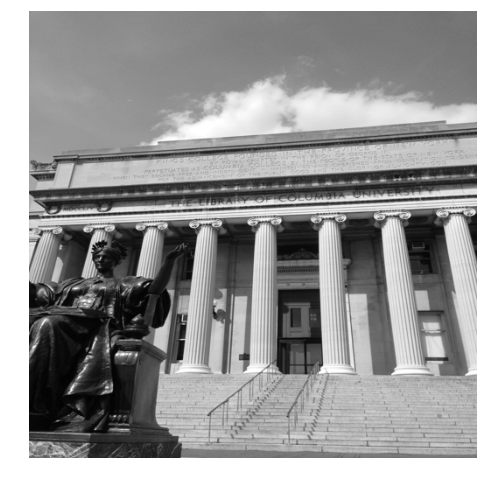
\includegraphics[width=65mm]{figures/columbia1.png}
&
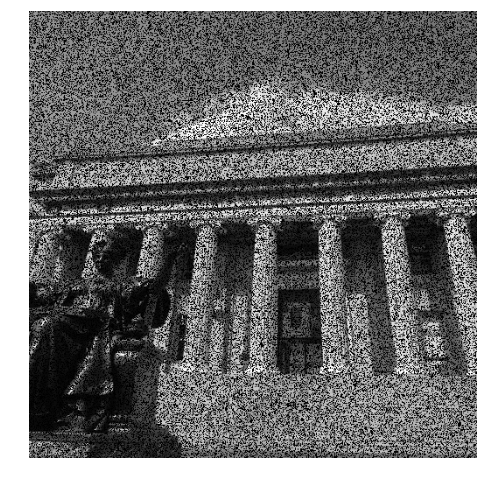
\includegraphics[width=65mm]{figures/columbia2.png}

&
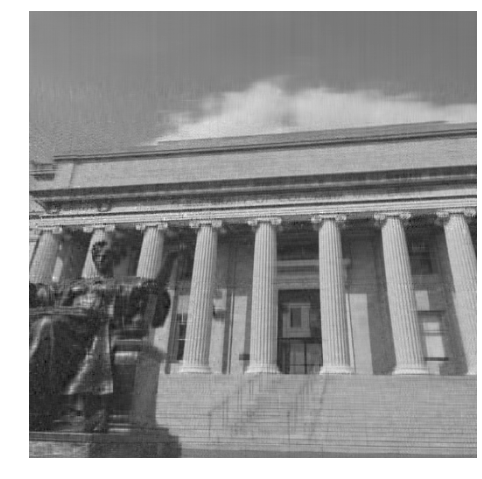
\includegraphics[width=65mm]{figures/columbia3.png}

\\

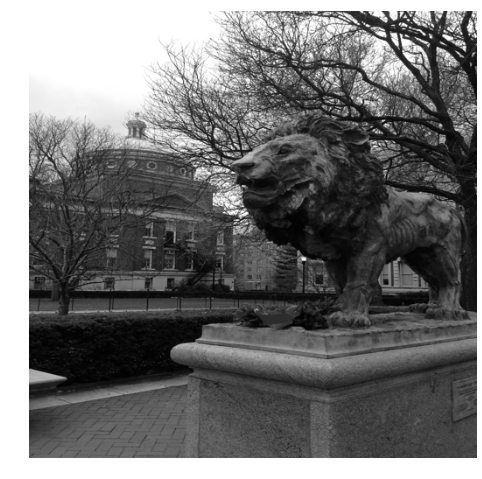
\includegraphics[width=65mm]{figures/columbia4.png}
&
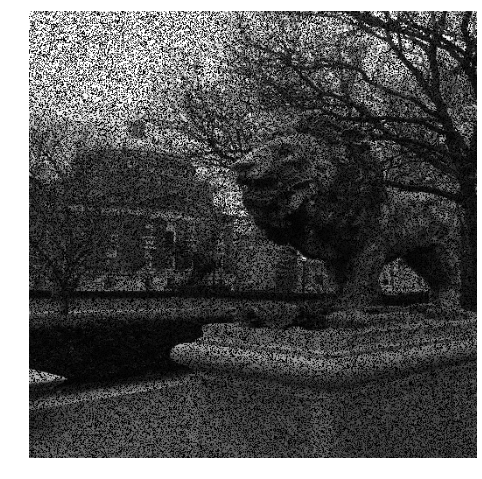
\includegraphics[width=65mm]{figures/columbia5.png}
&
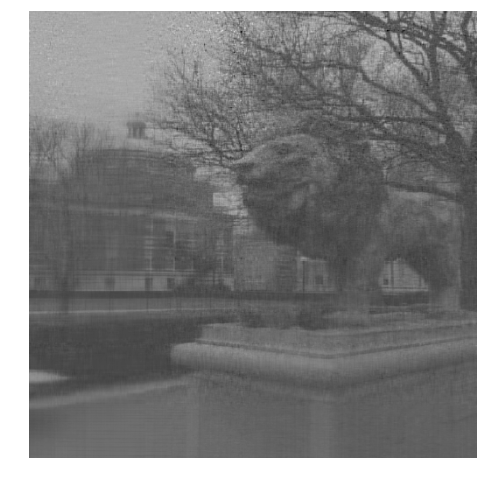
\includegraphics[width=65mm]{figures/columbia6.png}
\\

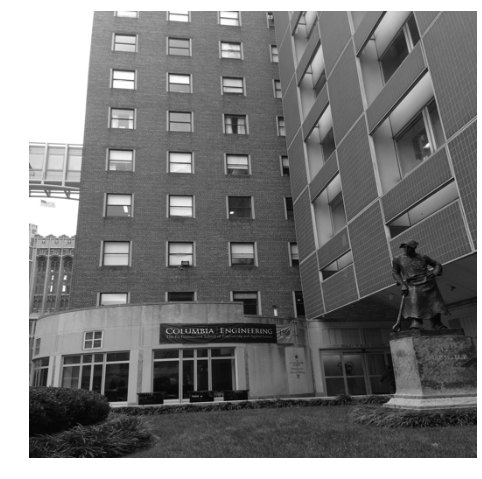
\includegraphics[width=65mm]{figures/columbia7.png}
&
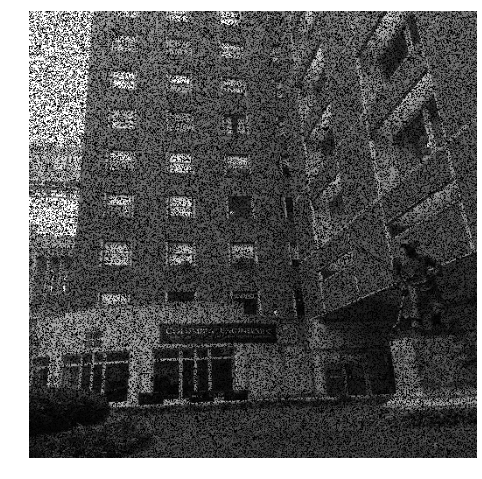
\includegraphics[width=65mm]{figures/columbia8.png}
&
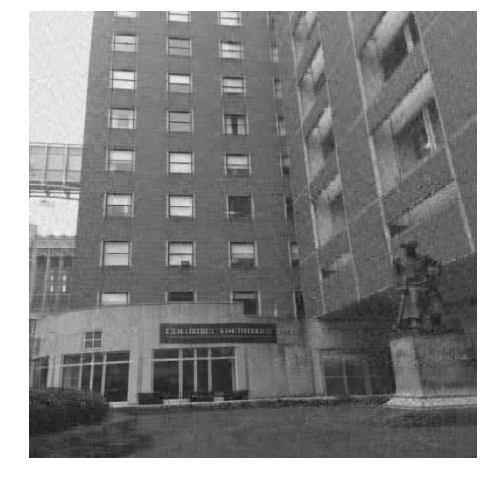
\includegraphics[width=65mm]{figures/columbia9.png}
\\
\end{tabular}

}

\caption{ASD method applied three different Columbia University images}
\end{figure}

\newpage



\section{Future Work}

We have plans for various improvements as we continue working with the \texttt{CompleteThat} python package. Overall, we would like to test the software and integrate automated testing cases into the software developing cycle. Also, documentation for the package and its functions, including examples, is high in our priority list. In addition, we hope to incorporate more rigorous error checking and make   available more customization to the user. 

For the memory-based algorithms it is well know that noise in the data introduces overfitting on the estimated matrix. Following the approach taken by Mazumder et al.~\cite{mazumder:2010}  where they solve the same objetive function as the problems above (using the Frobenious norm) but introducing the nuclear norm as regularizer to account for overfitting, we would introduce a regularization option into the matrix completion procedure. 

For the stochastic gradient descent method, we plan to add a lambda penalty feature for combatting overfitting as well as considering options for more advanced versions of our basic latent factor model as demonstrated by Koren~\cite{koren:2008} in his paper on the prize-winning Netflix models. 
For all algorithms, we would like to explore and research various hardware and software optimization techniques for faster code. 

Finally, given the similarities between matrix completion and robust principal component analysis one further extension to the functionality of the package could be implementing the robust-PCA procedure outlined by Cand\'es~\cite{candes:2011}, et al.

\newpage
\bibliographystyle{alpha}
\bibliography{references}

\newpage
\section{Source code}
On the whole, the package directory structure looks like the Figure~\ref{fig:code_scheme}. In the following we present the source code for the package.
\begin{figure}[h!]
  \centering
    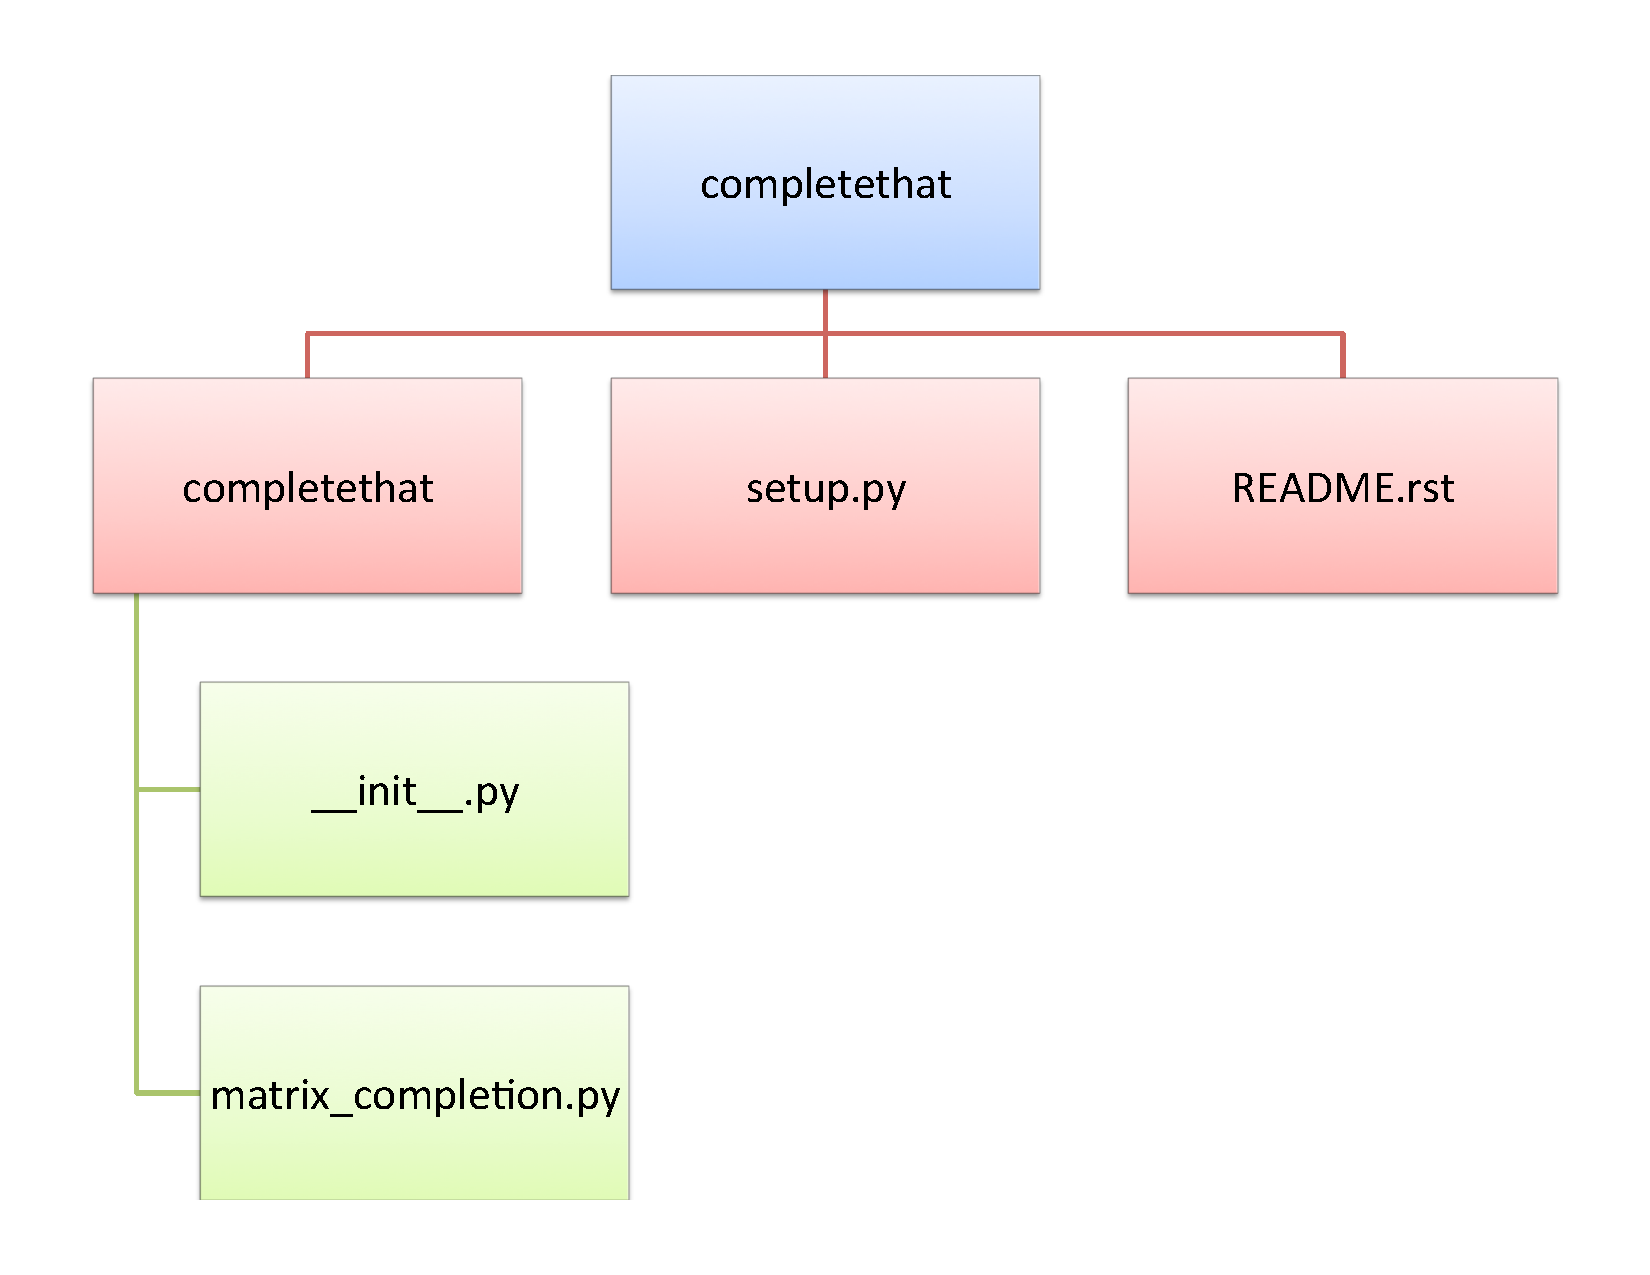
\includegraphics[width=0.8\textwidth]{./figures/code_scheme.pdf}
    \caption{CompleteThat structure}
    \label{fig:code_scheme}
\end{figure}

\code{completethat/matrix\_completion.py}{../code/completethat/matrix_completion.py}
\code{completethat/matrix\_\_init\_\_.py}{../code/completethat/__init__.py}
\code{completethat/matrix\_\_init\_\_.py}{../code/setup.py}



\newpage



\paragraph{Punctuation in equations.}
An equation is part of a sentence, and you may need to include a comma or a period
at the end of an equation as a result, whether or not you are using inline or
display math style. For example:
\begin{quote}
    We next discuss how to solve the problem
    \[
        \begin{array}{ll}
            \mbox{minimize} & (1/2)\|Ax - b\|_2^2,
        \end{array}
    \]
    where $x \in \reals^n$ is the optimization variable.
\end{quote}

\paragraph{Don't start a sentence with a symbol.}
This hurts readability:
\begin{quote}
Bad: $f$ is smooth.\\
Good: The function $f$ is smooth.

Bad: $x^n - a$ has $n$ distinct zeros. \\
Good: The polynomial $x^n - a$ has $n$ distinct zeros.
\end{quote}
Similarly, don't start a sentence with a reference.

\paragraph{Use words to separate symbols in different formulas.}
If it might confuse the reader visually or in the actual
meaning of the sentence, use words to break apart formulas:
\begin{quote}
Bad: The sequences $x_1, x_2, \dots$, $y_1, y_2, \dots$ are Cauchy. \\
OK: The sequences $x_1, x_2, \dots,$ and $y_1, y_2, \dots,$ are Cauchy. \\
Good: The sequences $(x_i)$ and $(y_i)$ are Cauchy.

OK: The image of $S$ under $f$, $f(S) = \{ x \mid x \in S \}$, is convex. \\
Good: The image of $S$ under $f$, given by $f(S) = \{ x \mid x \in S \}$, is convex.
\end{quote}
Do not insert superfluous words if the meaning is clear.
\begin{quote}
Good: Consider the function $f + g + h$, where $f : \reals^n \to
\reals$, $g : \reals^m \to \reals$, and $h : \reals^p \to \symm^n$ are closed
proper convex.
\end{quote}

\paragraph{References.}
For internal references, use the \texttt{label} and \texttt{ref} commands.
\emph{Never} number or refer to an entity using a specific number,
as in ``Table~3.''
Refer to ``Table~\ref{t-ex1}'', ``\eqref{e-opt-prob}'' (an equation), and so on.
Only number equations that are important and should be emphasized or that you
specifically refer to elsewhere. Do not simply number all equations, and do not
number them randomly. A numbered equation draws the reader's attention, so it
should be used relatively sparingly. Use \verb+\S+ for section references, as in
\S\ref{s-content}.

For external references, you must use Bib\TeX. Use references like nouns or 
footnotes:
\begin{quote}
Good: One useful reference is \cite{BoV:04}. \\
Good: Interested readers may refer to Boyd and Vandenberghe \cite{BoV:04}.
\end{quote}

Your Bib\TeX\ source must be correct.  Unfortunately, many systems that export
Bib\TeX\ entries export very poor ones.  Bib\TeX\ ignores the \texttt{*.bib}
file's capitalization for articles (but not books). To force capitalization,
you must wrap the letter with curly braces.  The hyphen (-), en dash (--), and
em dash (---) are distinct punctuation marks that serve different purposes.
(And the minus sign is different from all three.) When specifying a page range
in references, use the en dash. For an example of escaping and using the en
dash, look at our Bib\TeX\ entry for \cite{Tref:2008}.

\paragraph{Do not italicize English in math mode.}
Mathematical symbols should be typeset in math mode:
write $Ax=b$, not Ax=b. This said, subscripts or
superscripts that derive from English (or any human language) should not be
italicized. For example, write $f_\mathrm{best}$, not $f_{best}$. The exception
is subscripts based on a single letter: refer
to a point that is the center of some set as $x_c$, not $x_{\mathrm{c}}$.
Similarly, use commands for special functions: use $\sin(x)$,
$\log(x)$, and $\exp(x)$, not $sin(x)$, $log(x)$, or $exp(x)$.

A really heinous example would be the following:
\begin{quote}
Consider the problem
\[
\begin{array}{ll}
minimize & f(Ax - b) \\
\end{array}
\]
where x is the optimization variable and A and b are problem data.
\end{quote}

\paragraph{Spacing.}
A blank line ends a paragraph. You shouldn't leave a blank line between an
equation and the following text unless you intend the equation to end the
paragraph. Write:
\begin{quote}
\begin{verbatim}
The image of $S$ under $f$,
\[
    f(S) = \{ f(x) \mid x \in S \},
\]
is convex.
\end{verbatim}
\end{quote}
Inserting extra blank lines before \verb+\[+ or after \verb+\]+ will result in
bad typesetting. However, the following is fine, since a new paragraph is called for:
\begin{quote}
\begin{verbatim}
The image of $S$ under $f$ is defined as
\[
    f(S) = \{ f(x) \mid x \in S \}.
\]

We now turn to a different topic.
\end{verbatim}
\end{quote}
Using a tab before \verb+f(S)+ inside the equation environment is
optional, but helps readability in the source.  Similar rules should be
followed for other environments like \texttt{quote}; see the source of this
document.

\paragraph{Use of notation and jargon.}
The correct and appropriate use of notation and jargon takes time to master.
The following should give you a sense of what to think about:

\begin{itemize}
\item Don't use the same notation for two different things. Conversely, be consistent
about notation for the same thing mentioned in two places: don't
say ``$A_j$ for $1 \leq j \leq n$'' in one place and ``$A_i$ for $i=1,\ldots,n$'' 
in another, or use two different indices in summations over the same ranges. 
Formally, the $i$ and $j$ are dummy variables with only that phrase as scope,
so these are technically correct, but it will confuse the reader.

\item It can be useful to choose names for indices so, for example, $i$
always varies from 1 to $m$ and $j$ always varies from 1 to $n$ (when
referencing something like the rows and columns of an $m \times n$ matrix).

\item Define all symbols before or near to where you use them.  A good rule is that
when you first use something, say, $X$, you should either define it immediately, or 
within the paragraph.   There are a few cases where it is acceptable to define it 
later, but you must say this explicitly, as in ``$X$ is the matrix of activation
levels, which we define below.''

\item A symbol like $f$ refers to a function, while $f(x)$ refers to a
function evaluated at a given point. Avoid sloppy writing like ``The function
$f(x)$ is convex.''
So-called `anonymous' functions defined inline are an exception to this rule,
as in ``the function $x^2 \cos x$ is a counterexample,'' though this should
be used only for simple functions.

\item Use typographic naming conventions like capital letters for sets, Greek
letters for dual variables, \emph{etc}.

\item Try to use mnemonic notation, so $x_c$ for a center point,
$c$ for a cost vector, $S$ for a generic set, $C$ for a convex set, $B$
for a ball, and so on. Note that there are conventions about
the use of different letters in mathematics that you should not ignore:
$i$, $j$, and $k$ are usually used for indices, $x$ through $z$ for
variables, $a$ through $d$ for constants, \emph{etc}.

\item Don't use symbols like $\forall$, $\exists$, and $\Rightarrow$; use the
corresponding words. These symbols are usually appropriate only in
formal logic. 

\item Don't overuse subscripts. If you do not need to assign a subscript
to something, don't. For example, if you begin by defining a set as
$X = \{x_1, \dots, x_n\}$, then it is going to get annoying to refer to subsets
of $X$, since you will need double subscripts. If possible, it would be better
to not name the elements of $X$ and only refer to them when necessary, just
as, say, $x$ and $y$. 

Beware especially of any topic in graph theory when it comes to this rule;
there are often \emph{many} ways to refer to relevant objects, and finding
reasonable notation can often get one half the way to getting a handle on the
problem itself.

\item Don't assign symbols to concepts that you never refer to, or can easily
refer to without:
\begin{quote}
Bad: Let $X$ be a compact subset of a space $Y$. If $f$ is a continuous
real-valued function over $X$, it has a minimum over $X$. \\
Good: A continuous real-valued function has a minimum over a compact set.
\end{quote}
Similarly, do not say ``The solution $x^\star$ is unique'' if you never need
to refer to $x^\star$ again; simply say that the solution is unique.
When you say ``The solution $x^\star$ is unique'' you are both stating a fact
\emph{and} entering the symbol $x^\star$ into the paper's symbol table and
the reader's working memory.
\end{itemize}

\paragraph*{Sections.}
Use structures like \texttt{section}, \texttt{subsection},
\texttt{subsubsection}, and \texttt{paragraph} to organize the exposition;
never insert manual line breaks or page breaks for this purpose. In particular,
do not use line breaks to separate different topics. Do not use symbols in
article titles and ideally not even in section headers.

\paragraph{Use capitalization consistently.}
For section headers, capitalize the first letter, proper nouns, and lowercase
everything else, as in this document.  For references, write Figure 1, Algorithm 3,
Theorem 4, and so on.

\paragraph{Use the right commands.}
There are certain special commands in \LaTeX\ for notation that you otherwise
might attempt to write in an ad-hoc manner. If you do the latter, the typesetting
will be inferior. A few common examples:
\begin{itemize}
\item Norms are written $\|x\|$, not $||x||$. 

\item For set-builder notation, use
$\{ x \in \reals \mid x \geq 0 \}$, not $\{x \in \reals | x \geq 0 \}$.

\item Make sure to use \verb+\left+ and \verb+\right+ when wrapping
taller expressions with parentheses, curly braces, brackets, and so on.
\begin{quote}
Bad: Let
\[
    x = \argmin_u (f(u) + \frac{1}{2}\|u - z\|_2^2).
\]
Good: Let
\[
    x = \argmin_u \left(f(u) + \frac{1}{2}\|u - z\|_2^2\right).
\]
\end{quote}

\item Use \verb+\ldots+ (lower dots) when the dots are surrounded by commas and
\verb+\cdots+ (center dots) when surrounded by other objects that have full
height, as in $x_1, x_2, \ldots, x_n$ and $x_1 + x_2 + \cdots + x_n$.
\end{itemize}
Similarly, make sure to use our conventions for standard mathematical objects
for this class; for example, use $\reals$, not $\mathbb{R}$, to denote the set
of real numbers. Use the \verb+\argmin+ and \verb+\argmax+ commands (as shown
above); do not write `arg min', since `argmin' is a single mathematical
operator.  These and other definitions are provided in \verb+defs.tex+.

\paragraph{Writing optimization problems.}
In this class, optimization problems can be introduced in the sentence as
nouns. For example, write as follows:
\begin{quote}
Consider the problem
    \begin{equation}
    \begin{array}{ll}
    \mbox{minimize}   & (1/2)\|Ax-b\|_2^2 + \lambda \|x\|_1 \\
    \mbox{subject to} & 0 \preceq x \preceq \ones \\
    & \|x\|_2 \leq 1,
    \end{array}
    \label{e-opt-prob}
    \end{equation}
where $x \in \reals^n$ is the optimization variable, and $A \in \reals^{m
\times n}$, $b \in \reals^m$, and $\lambda > 0$ are problem data.
\end{quote}
It is important to state which symbols refer to variables and which to problem data.

Be sure to carefully distinguish an optimization problem, 
an algorithm for solving it, and its optimal value.
You \emph{solve} a problem (possibly, using a particular algorithm);
an optimization problem \emph{has} an optimal value;
and an optimization problem \emph{is} convex, or infeasible.
It does not make sense to talk about whether or not a problem converges.



\label{s-content}





\end{document}
